	Con el objetivo de hallar los parámetros característicos del cirucito \textit{slew rate} y ancho de banda, se simula la respuesta al escalón para dos casos, pequeña y gran señal.

\subsection{Respuesta la escalón para pequeña señal}

\HgraficarPNG{0.5}{sim_rta_escalon_peque.png}{Respuesta al escalón en pequeña señal.}{fig:rta_escalon_peque}

\subsection{Respuesta al escalón para gran señal}

\begin{figure}[H]
	\centering
	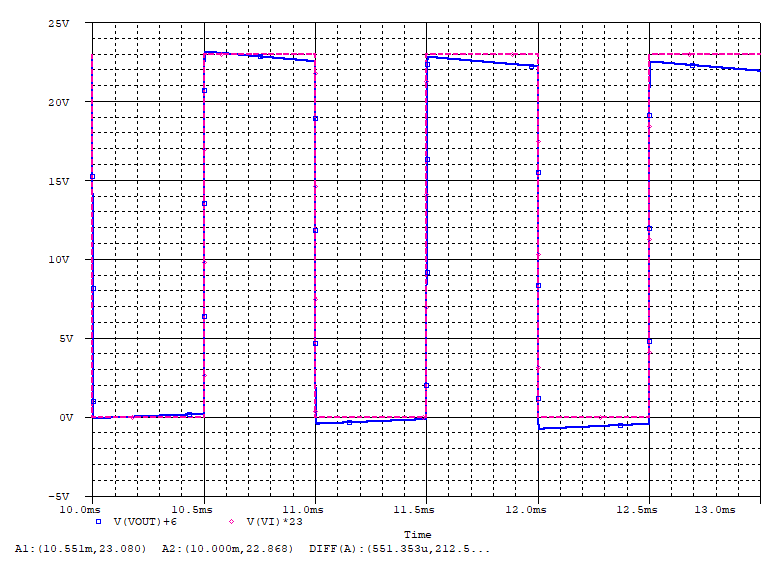
\includegraphics[scale=0.5]{sim_rta_escalon_gran.png}
	\caption{Respuesta al escalón en gran señal}
	\label{fig:rta_escalon_gran}
\end{figure}
%\HgraficarPNG{0.5}{sim_rta_escalon_gran.png}{Respuesta al escalón en gran señal.}{fig:rta_escalon_gran}

	En las Figuras \ref{fig:rta_escalon_peque} y \ref{fig:rta_escalon_gran} se muestra la respuesta al circuito ante ante una señal cuadrada de frecuencia \SI{1}{\kilo\hertz} y amplitud $1\hat{V}$ y $10m\hat{V}$ respectivamente. Se puede observar en ambos casos que el circuito se encuentra correctamente compensado debido a la ausencia de sobrepicos de tensión u oscilaciones (tal como se mostró en la elección del capacitor de compensación, Figura \ref{fig:var_cap}). 
	
	Si bien el modelo de simulación involucra capacidades parásitas, en la práctica éstas pueden diferir, por lo que es posible que el valor del capacitor de compensación deba ser cambiado, buscando un equilibrio entre los valores de  slew rate y ancho de banda.
	
	A continuación se calculan los valores de \textit{slew rate} y ancho de banda en base a lo simulado.
\subsection{Ancho de banda}

	Este parámetro se obtiene a partir de la simulación de la respuesta al escalón del circuito en pequeña señal (\SI{10}{\milli\volt}).
	
	\HgraficarPNG{0.5}{sim_rta_escalon_gran_zoom.png}{Respuesta al escalón en pequeña señal.}{fig:rta_escalon_peque}

%\begin{figure}[H]
%	\centering
%	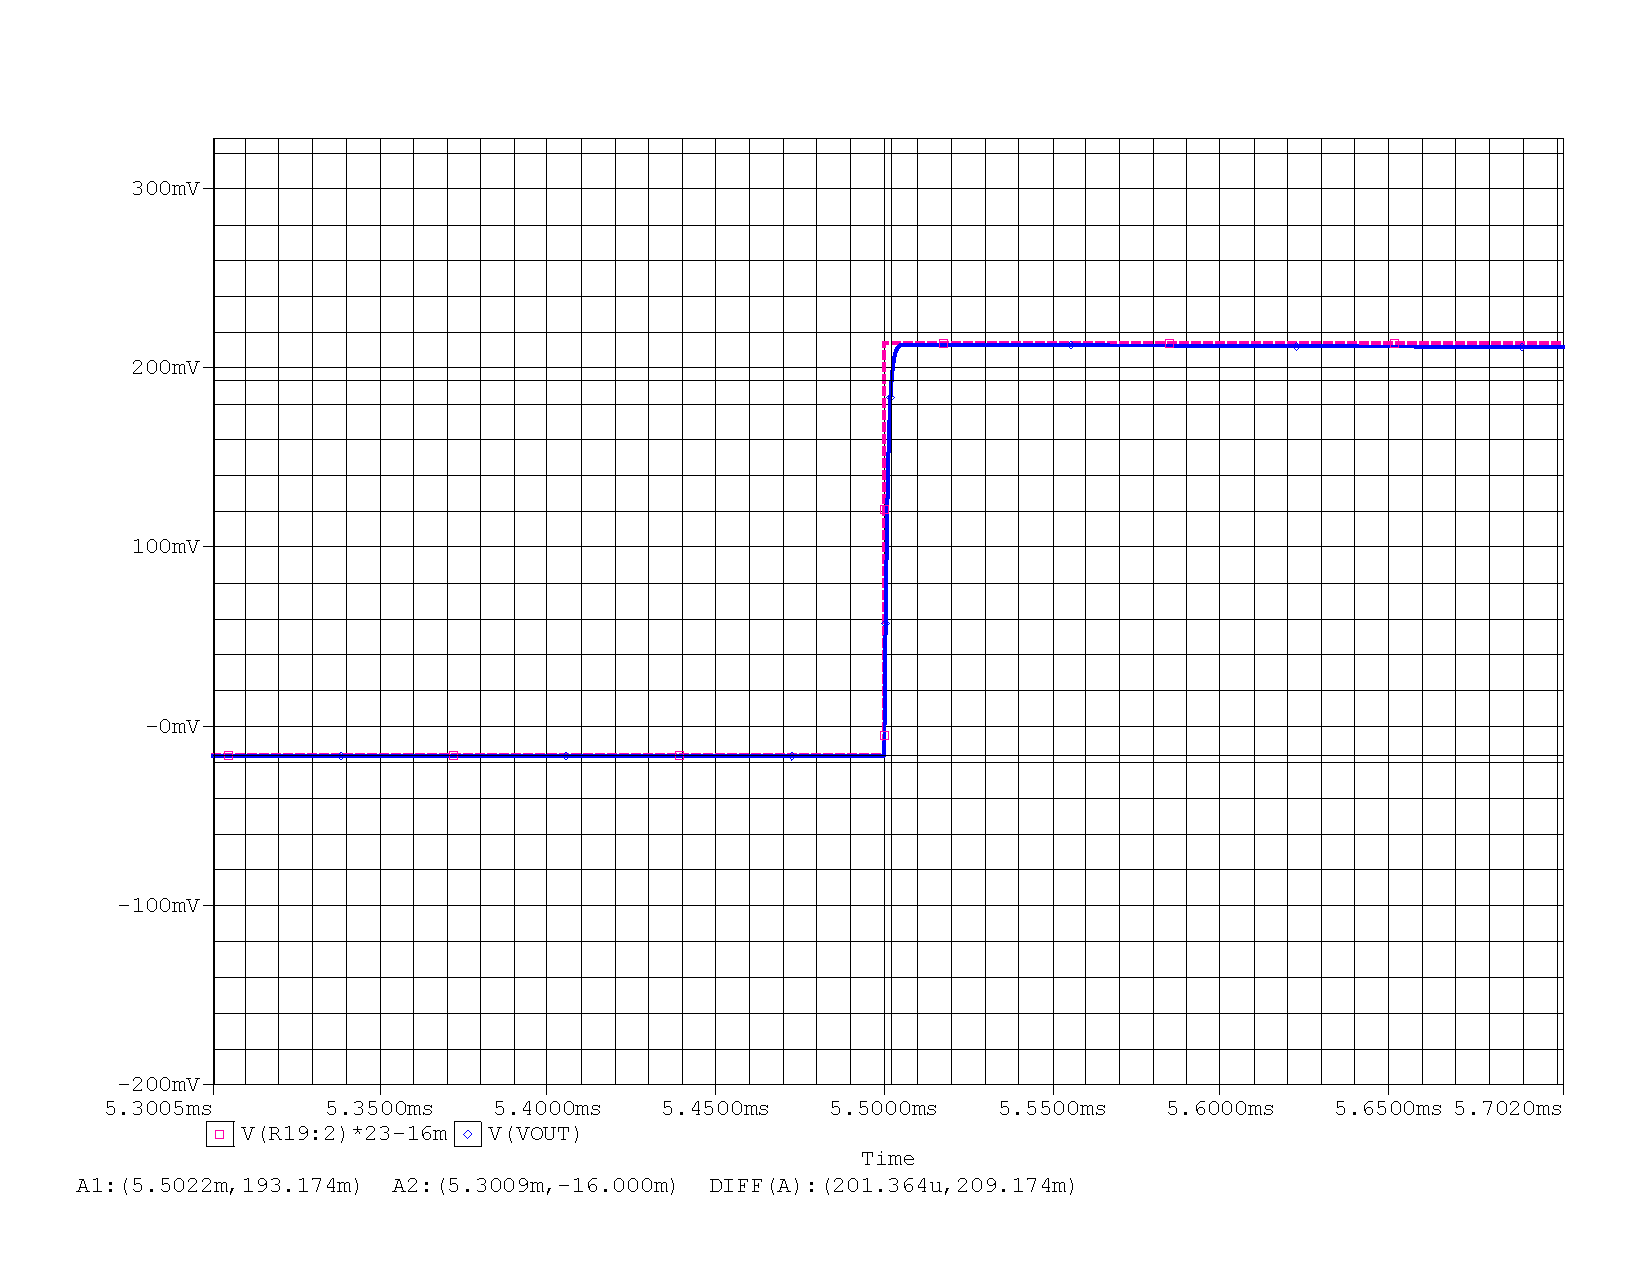
\includegraphics[scale=0.4]{sim_rta_escalon_senial_peque_zoom.pdf}
% 	\caption{Respuesta al escalón en pequeña señal.}
%	\label{fig:rta_escalon_peque}
%\end{figure}

	Observando la Figura \ref{fig:sim_bw} el tiempo de crecimiento ($\tau_r$), se puede determinar el ancho de banda mediante la ecuación \eqref{ec:bw}.

	\begin{equation}
		\centering
		\mathrm{BW} = \frac{\num{0,35}}{\tau_r} = \frac{0,35}{\SI{2}{\micro\second}} = \boxed{\SI{175}{\kilo\hertz}}
		\label{ec:bw}
	\end{equation}

\subsection{\textit{Slew Rate}}

\HgraficarPNG{0.5}{sim_rta_escalon_gran_zoom.png}{Respuesta al escalón en gran señal ampliado.}{fig:sim_rta_escalon_gran_sr}

%\begin{figure}[H]
%	\centering
%	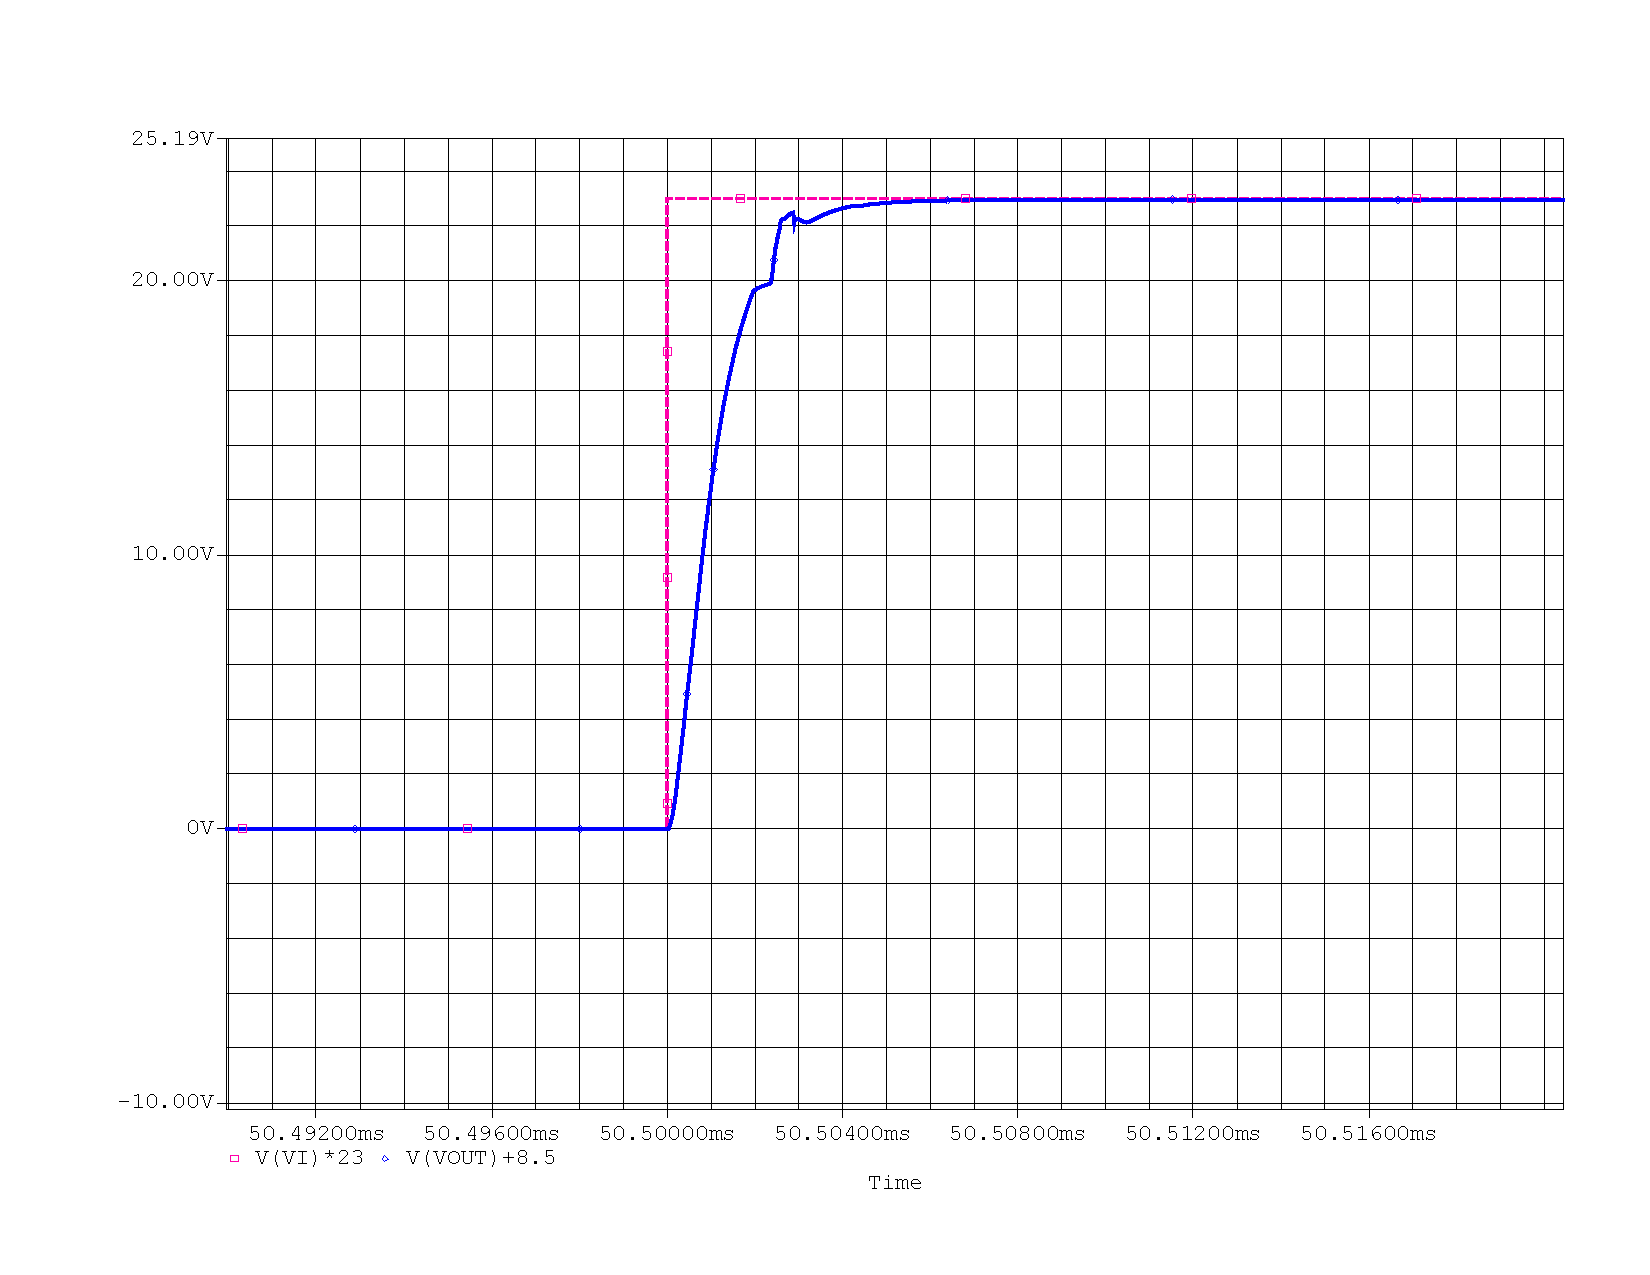
\includegraphics[scale=0.4]{sim_rta_escalon_gran_senial_zoom_sr.pdf}
%	\caption{Respuesta al escalón en gran señal ampliado.}
%	\label{fig:sim_rta_escalon_gran_sr}
%\end{figure}
	
	El parámetro \textit{Slew Rate} caracteriza el comportamiento de la salida del circuito ante cambios súbitos de tensión en la entrada, ya que la tensión de salida no puede responder de forma instantánea ante alteraciones en la entrada. Para hallar su valor se impone un escalón en la entrada de gran amplitud y se mide la pendiente casi constante resultante. A partir de la Figura \ref{fig:sim_rta_escalon_gran_sr} se obtiene \eqref{ec:sr}.

	\begin{equation}
	\centering
	\mathrm{SR} = \left. \frac{dV_o(t)}{dt} \right\rvert_{max} \cong \frac{\Delta V_o}{\Delta t} = \frac{\SI{27}{\volt}}{\SI{3}{\micro\second}} = \boxed{\SI{9}{\volt\per\micro\second}}
	\label{ec:sr}
\end{equation}


A partir del parámetro obtenido se puede calcular la máxima frecuencia para la cual el amplificador es capaz de reproducir la máxima amplitud de salida sin deformación.

\begin{equation}
	\centering
	f = \frac{SR}{2 \cdot \pi \hat{V} } = \frac{\SI{9}{\volt\per\micro\second}}{2 \cdot \pi \SI{26}{\volt}} = \SI{55}{\kilo\hertz}
	\label{ec.max_f}
\end{equation}

Se realizó una simulación con una señal de entrada de $1 \hat{V}$ a frecuencia $\SI{55}{\kilo\hertz}$, la salida obtenida se muestra en la Figura \ref{fig.sim_55k_alta}. La distorsión resultó ser $THD = \num{2.6}\%$, y es debida a los transistores de conmutación. 

\HgraficarPNG{0.5}{sim_55k_alta_26}{Simulación a máxima tensión de salida y \SI{55}{\kilo\hertz}.}{fig.sim_55k_alta}

	Se probó con una frecuencia de \SI{25}{\kilo\hertz} a máxima tensión de salida, y se obtuvo una $THD=\num{0.2}\%$, y a $\SI{20}{\kilo\hertz}$ $THD=\num{0.099}\%$. Dichos resultados se encuentran dentro de los valores especificados, ya que al tratarse de un amplificador de audio, la máxima frecuencia audible es como mucho \SI{20}{\kilo\hertz}.

\HgraficarPNG{0.5}{sim_25k_02}{Simulación a máxima tensión de salida y \SI{25}{\kilo\hertz}.}{fig.sim_25k_alta}


Asimismo se debe destacar que la distorsión a \SI{55}{\kilo\hertz} resulta mucho menor para amplitudes de señal que no logran conmutar. Por ejemplo, en la Figura \ref{fig.sim_salida_55k_baja} se muestra la simulación para una salida de $\num{4.5}\hat{V}$ y se obtuvo una distorsión de $THD=\num{0.03}\%$. Se puede apreciar el efecto del \textit{slew rate} por la forma de las puntas de la señal que empiezan a formar rectas. Dicho efecto será más pronunciado al aumentar la frecuencia.

\HgraficarPNG{0.5}{sim_55k_vo_baja_03}{Salida a \SI{55}{\kilo\hertz}.}{fig.sim_salida_55k_baja}


En resumen, para cualquier amplitud de señal de salida (hasta $26\hat{V}$), la señal puede ser reproducida correctamente hasta \SI{25}{\kilo\hertz}.

